\documentclass[a4paper]{extarticle}

% Encoding and fonts
\usepackage[utf8]{inputenc}
\usepackage[T1]{fontenc}
\usepackage{lmodern}
\usepackage{xcolor}      % For color definitions
\usepackage{tcolorbox}   % For colored boxes
% Page layout
\usepackage[margin=1in]{geometry}

% Math packages
\usepackage{amsmath, amssymb, amsthm}

% Graphics and plots
\usepackage{tikz}
\usepackage{pgfplots}
\pgfplotsset{compat=newest}

% Additional utilities
\usepackage{etoolbox}
\usepackage{microtype}

% Patching pgfplots warning
\makeatletter
\patchcmd{\pgfplots@applistXXpushback@smallbuf}{\pgfplots@error}{\pgfplots@warning}{}{}
\makeatother

% Theorem and color box settings
\usepackage{tcolorbox}
\tcbuselibrary{theorems}

\newtcolorbox{definitionbox}{
  title=Definition,
  fonttitle=\bfseries,
  colback=blue!5!white,
  colframe=blue!30!white,
  coltitle=black,
  boxrule=1.5pt,
  arc=3pt,
  outer arc=3pt,
}

\newtcolorbox{proofbox}{
  title=Proof,
  fonttitle=\bfseries,
  colback=custom_blue!20!white,
  colframe=custom_blue,
  coltitle=white,
  boxrule=0.5pt,
  arc=4pt,
  outer arc=4pt,
}

% Theorem box
\newtcolorbox{theorembox}{
  title=Theorem,
  fonttitle=\bfseries,
  colback=custom_green!30!white,
  colframe=custom_green,
  coltitle=black,
  boxrule=0.5pt,
  arc=4pt,
  outer arc=4pt,
}

\newtcolorbox{notebox}{
  title=Note,
  fonttitle=\bfseries,
  colback=red!5!white,
  colframe=red!30!white,
  coltitle=black,
  boxrule=0.5pt,
  arc=4pt,
  outer arc=4pt,
}


\definecolor{custom_green}{HTML}{a3be8c}
\definecolor{custom_red}{HTML}{bf616a}
\definecolor{custom_blue}{HTML}{5e81ac}


\newtcolorbox{examplebox}[1][]{
  title=#1,
  fonttitle=\bfseries,
  colback=custom_red!20!white,
  colframe=custom_red,
  coltitle=white,
  boxrule=0.5pt,
  arc=4pt,
  outer arc=4pt,
}

\theoremstyle{definition}
\newtheorem{definition}{Definition}[section]
\newtheorem{example}[definition]{Example}

\theoremstyle{plain}
\newtheorem{theorem}[definition]{Theorem}

\title{
Mathematical Methods II\\[2ex]
Exams:\\
70\% Exam\\
30\% Continuous Assessment (3 parts)
}
\author{}
\date{}

\begin{document}
\maketitle
\pagebreak

\tableofcontents
\pagebreak

\section{Week 1: Intro to Laplace Transforms}

\subsection{Table of Laplace Transforms}
\[
  \begin{array}{|c|c|}
    \hline
    f(t)                   & \mathcal{L}\{f(t)\}               \\ \hline
    1                      & \frac{1}{s}, \, s > 0             \\ \hline
    t                      & \frac{1}{s^2}, \, s > 0           \\ \hline
    t^n, \, n = 0, 1, 2, 3 & \frac{n!}{s^{n+1}}, \, s > 0      \\ \hline
    e^{at}                 & \frac{1}{s-a}, \, s > a           \\ \hline
    \cos(\omega t)         & \frac{s}{s^2 + \omega^2}          \\ \hline
    \sin(\omega t)         & \frac{\omega}{s^2 + \omega^2}     \\ \hline
    \cosh(at)              & \frac{s}{s^2 - a^2}, \, s > |a|   \\ \hline
    \sinh(at)              & \frac{a}{s^2 - a^2}, \, s > |a|   \\ \hline
    e^{at} \cos(\omega t)  & \frac{s-a}{(s-a)^2 + \omega^2}    \\ \hline
    e^{at} \sin(\omega t)  & \frac{\omega}{(s-a)^2 + \omega^2} \\ \hline
    e^{at} f(t)            & F(s-a)                            \\ \hline
  \end{array}
\]
\subsection{Preliminary: Exponential Functions}
Recall the following facts:
\begin{enumerate}
  \item \( e^t = \exp(t) = 1 + \frac{t^1}{1!} + \frac{t^2}{2!} + \frac{t^3}{3!} + \cdots
        = \sum_{i=0}^\infty \frac{t^i}{i!}.\)
  \item \( e^0 = 1.\)
  \item As \( t \to \infty \), \( e^t \to \infty \);\quad as \( t \to -\infty \), \( e^t \to 0.\)
  \item \(\frac{d}{dt}\, e^t = e^t\),\quad and\quad \(\frac{d}{dt}\, e^{st} = s\, e^{st}.\)
  \item \(\displaystyle \int e^t\, dt = e^t + C,\quad \text{and} \quad
        \int e^{st}\, dt = \frac{1}{s}\, e^{st} + C.\)
  \item \( e^{t_1} \cdot e^{t_2} = e^{\,t_1 + t_2}.\)
\end{enumerate}

\subsection{Laplace Transforms}

\begin{definitionbox}
  Consider a function \(f(t)\) for \(t > 0\).\\[1ex]
  We define the Laplace transform of \(f(t)\) as
  \[
    \mathcal{L}\{f(t)\} = \int_0^\infty e^{-st} f(t) \, dt.
  \]
\end{definitionbox}

\begin{notebox}
  We can also write \( \mathcal{L}\{f(t)\} \) as \( F(s) \).\\[1ex]
  Alternatively,
  \[
    \mathcal{L}\{f(t)\} = \lim_{R \to \infty} \int_0^R e^{-st} f(t) \, dt.
  \]
\end{notebox}

\noindent Recalling that

$$\int_0^1 s t^2 \, dt = s\Big[\frac{t^3}{3}\Big]_0^1 = \frac{s}{3}$$

\noindent we see that \( \mathcal{L}\{f(t)\} \) is just a function of \( s \).

\pagebreak
\subsection{Laplace Transforms of Common Functions}
Given the function \( f(t) \), its Laplace transform is denoted as:
\[
  \mathcal{L}\{f(t)\} = \int_0^\infty e^{-st} f(t) \, dt.
\]
\begin{notebox}
  \begin{align*}
    \mathcal{L}\{1\} = \int_{0}^{\infty} e^{-st} \, dt
     & = \left[\dfrac{e^{-st}}{-s}\right]_0^\infty \\
  \end{align*}
  At \(t = 0\), \(e^{-st} = 1\) and as \(t \to \infty\), \(e^{-st} = 0\), so

  \[
    \mathcal{L}\{1\} = \left(0 - \frac{1}{-s}\right) = \frac{1}{s} \quad s > 0
  \]

\end{notebox}

\begin{notebox}
  \begin{align*}
    \mathcal{L}\{e^{kt}\}
     & = \int_{0}^{\infty} e^{-st} e^{kt} \, dt           \\[6pt]
     & = \int_{0}^{\infty} e^{(k-s)t} \, dt               \\[6pt]
     & = \left[\frac{e^{(k-s)t}}{k-s}\right]_{0}^{\infty}
  \end{align*}

  As \(t \to \infty\), \(e^{(k-s)t} = 0\), and at \(t = 0\), \(e^{(k-s)t} = 1\).\\
  Applying the limits:
  \begin{align*}
    \left[\dfrac{e^{(k-s)t}}{k-s}\right]_0^\infty
     & = \dfrac{0}{k-s} - \dfrac{1}{k-s}        \\[6pt]
     & = -\dfrac{1}{k-s}                        \\[6pt]
     & = \dfrac{1}{s-k} \quad \text{for } s > k
  \end{align*}

  Thus,
  \[
    \mathcal{L}\{e^{kt}\} = \dfrac{1}{s-k}, \quad s > k
  \]
\end{notebox}

\begin{notebox}
  \begin{align*}
    \mathcal{L}\{a f(t) + b g(t)\}
     & = \int_{0}^{\infty} e^{-st} \Big(a f(t) + b g(t)\Big) \, dt \\[6pt]
     & = a \int_{0}^{\infty} e^{-st} f(t) \, dt
    + b \int_{0}^{\infty} e^{-st} g(t) \, dt                       \\[6pt]
     & = a\,\mathcal{L}\{f(t)\} + b\,\mathcal{L}\{g(t)\}.
  \end{align*}
\end{notebox}
\newpage
\section{Week 2 : Laplace Transforms of Hyperbolic Functions}
Last week we saw:
\begin{itemize}
  \setlength\itemsep{1pt}
  \item \(\mathcal{L}\{1\} = \dfrac{1}{s}\)
  \item \(\mathcal{L}\{e^{kt}\} = \dfrac{1}{s-k}\)
  \item \(\mathcal{L}\{a f(t) + b g(t)\} = a\,\mathcal{L}\{f(t)\} + b\,\mathcal{L}\{g(t)\}\)
\end{itemize}
\subsection{Laplace Transforms of Hyperbolic Functions}
Recall:
\begin{figure}[htbp]
  \centering
  \begin{minipage}[c]{0.45\textwidth}
    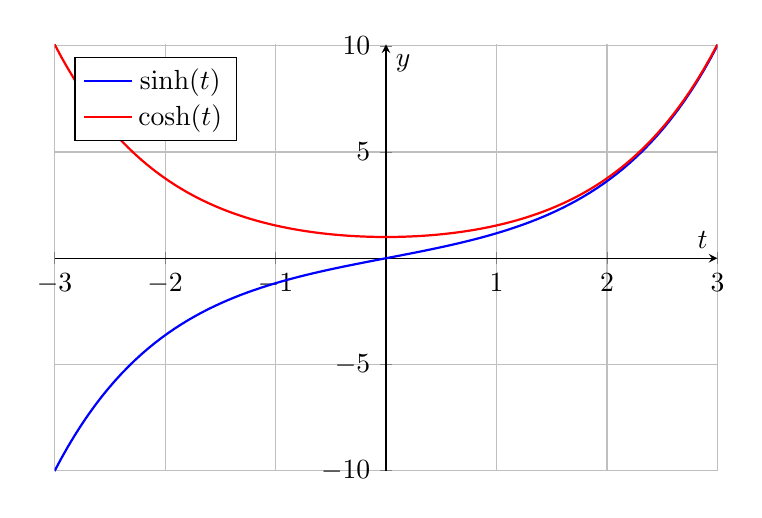
\begin{tikzpicture}
      \begin{axis}[
          axis lines=middle,
          xlabel={$t$},
          ylabel={$y$},
          domain=-3:3,
          samples=100,
          width=10cm,
          height=7cm,
          grid=both,
          legend pos=north west
        ]
        % Plot sinh(t)
        \addplot [blue, thick] {sinh(x)};
        \addlegendentry{$\sinh(t)$}
        % Plot cosh(t)
        \addplot [red, thick] {cosh(x)};
        \addlegendentry{$\cosh(t)$}
      \end{axis}
    \end{tikzpicture}
  \end{minipage}%
  \hfill
  \begin{minipage}[c]{0.45\textwidth}
    \begin{itemize}
      \item \( \cosh(t) = \frac{e^t + e^{-t}}{2} \).
      \item \( \sinh(t) = \frac{e^t - e^{-t}}{2} \).
      \item \( \tanh(t) = \frac{\sinh(t)}{\cosh(t)} \).
    \end{itemize}
  \end{minipage}
\end{figure}

\begin{examplebox}[Example]
  Find the Laplace Transofrm of $f(t) = \cosh(5),  t > 0$
  \begin{align*}
    \mathcal{L}\{\cosh(5t)\} & = L\left\{\dfrac{e^{5t} + e^{-5t}}{2}\right\}               \\
                             & = \dfrac{1}{2} \left(L\{e^{5t}\} + L\{e^{-5t}\}\right)      \\
                             & = \dfrac{1}{2} \left(\dfrac{1}{s-5} + \dfrac{1}{s+5}\right) \\
                             & = \dfrac{1}{2} \left(\dfrac{s+5 + s-5}{s^2 - 25}\right)     \\
                             & = \dfrac{1}{s^2 - 25}
  \end{align*}
  \noindent Similarly: The Laplace Transofrm of $\cosh{at}$ is: $$\dfrac{s}{s^2 - a^2}$$.
\end{examplebox}

\begin{examplebox}[Example]
  Find the Laplace Transorm of $\cos(\omega t)$ and $i\sin(wt)$, where $w  \text{ is a const.}$ and  $t > 0$. \\
  Recall \textbf{De Moivre's Theorem}:
  $$e^{iwt} = \cos(wt) + i\sin(wt)$$
  Here: $\mathcal{L}\{e^{iwt}\} = \frac{1}{s-iw}, \quad \text{with} \; k = iw$
\end{examplebox}

\newpage
\subsection{First Shift Theorem}
\begin{theorembox}
  If $f(t)$ has a Laplace Transform $F(s)$, defined for $s > k$, then $e^{at}f(t)$ has transform $F(s-a)$, defined for $s-a > k$, that is:
  $$\mathcal{L}\{e^{at}f(t)\} = F(s-a)$$
  or, taking the inverse on both sides:
  $$e^{at}f(t) = \mathcal{L}^{-1}\{F(s-a)\}$$
\end{theorembox}
\begin{proofbox}
  From the definition of the Laplace Transform:
  $$\mathcal{L}\{e^{at}f(t)\} = \int_0^\infty e^{-st}[e^{at}f(t)] \, dt =  \int_0^\infty e^{-(s-a)t} f(t) \, dt = F(s-a)$$
  We see, if $\mathcal{L}\{f(t)\}$ exists for $s > k$, then $\mathcal{L}\{e^{at}f(t)\}$ exists for $s > k + a$.
\end{proofbox}

\begin{examplebox}[Example]
  Find the Laplace Transform of $e^{at} \cos(\omega t)$
  We recalll that:
  $$\mathcal{L}\{\cos(\omega t)\} = F(s), \quad \text{where} \; F(S) = \dfrac{s}{s^2 + \omega ^2}$$
  Hence, using the first shift theorem above, we have:
  $$\mathcal{L}\{e^{at} \cos(\omega t)\} = F(s-a) = \dfrac{s-a}{(s-a)^2 + \omega^2}$$
\end{examplebox}
\end{document}
